\chapter{Empirical Evaluation} \label{ch:empirical}

In this chapter, we conduct an empirical evaluation of the CP compiler. We
analyze the impact of various optimizations in the CP compiler. Furthermore, we
compare the efficiency of dynamic inheritance in CP with that in handwritten
JavaScript code. The key takeaway from our empirical evaluation is that using a
naive compilation scheme for merges can be orders of magnitude slower than
optimized code. Our optimizations lead to code that can be competitive with
similar handwritten JavaScript code. The benchmarks are available in the
supplementary materials.

\paragraph{Experimental setup and benchmark programs.}
We performed experiments on a system featuring an Apple M1 Pro chip and 16GB
RAM. JavaScript code was executed using Node.js 20.12.2 LTS. The outline of
benchmark programs is presented in \autoref{tab:benchmark}. The initial four
benchmarks focus on general-purpose computations, while the latter four are
adapted from examples in \autoref{ch:embedding}, showcasing CP's novel features.
Among them, \textsf{chart} is the biggest program with around 300 lines of code.
Challenges discussed in \autoref{sec:overview}, including dynamic inheritance
and family polymorphism, are prominent in the latter four benchmarks.

\section{Ablation Study on Optimizations} \label{sec:optimization}

The coercive subtyping semantics of CP raises important questions about
efficiency since coercions have runtime costs and they are pervasively employed
in generated code. There are essentially three main concerns that need to be
addressed in obtaining an efficient compilation scheme for CP:

\begin{itemize}

\item \textbf{Efficient lookup.} Since merge lookup is pervasive, it is
      important to use a runtime representation for merges that enables
      efficient lookup.

\item \textbf{Efficient merging and copying.} Since merging is frequent, it is
      important that the merging process is efficient and minimizes the amount
      of copying involved in merging.

\item \textbf{Minimizing the cost of coercions.} Since our subtyping is
      coercive, it is fundamental that the cost of coercions is minimized.
      Furthermore, optimizations should avoid coercions when possible.
  
\end{itemize}

\noindent
In our work, we have addressed the above three points. Our representation of
merges as type-indexed records makes the cost of a merge lookup essentially the
same as the cost of a JavaScript field lookup, which is very efficient. This
provides a major source of improvement over a representation with pairs, where
lookup time can be linear. We believe that it is hard to do better in this
dimension, at least if the goal is to target JavaScript. For merging, we rely on
JavaScript's ability to copy object fields. An important concern for merging is
to avoid the creation of intermediate objects, minimizing the amount of copying.
The DPS optimization is particularly important for obtaining efficient merging.
Like lookup, we believe that the CP compiler also achieves efficient merging.
Finally, to mitigate coercions, we employ a hybrid model that combines inclusive
and coercive subtyping. We only insert coercions when necessary and try to
eliminate redundant coercions as much as possible. We have mentioned several
optimizations in \autoref{ch:compilation}, two of which are avoiding unnecessary
coercions: one for equivalent types and the other for record projections.

All the implemented optimizations should improve the performance of our CP
compiler in theory. Here we select four representative ones to evaluate their
impact in practice:
\begin{enumerate}
\item Reducing intermediate objects using destination-passing style (\textsf{DPS});
\item Preventing primitive values from boxing/unboxing (\textsf{NoBox});
\item Eliminating coercions for subtyping between equivalent types (\textsf{TyEquiv} \& \textsf{CoElim});
\item Avoiding the insertion of coercions for record projections (\textsf{ProjOptim}).
\end{enumerate}

\begin{table}
\caption{Outline of the benchmark programs.$^\dagger$} \label{tab:benchmark}
\centering
\footnotesize
\begin{tabular}{r l}
\toprule
\sffamily \bfseries fib & Calculating Fibonacci numbers without memoization. \\
\midrule
\sffamily \bfseries fact & Some factorial functions multiplied together. \\
\midrule
\sffamily \bfseries sieve & Sieve of Eratosthenes, an algorithm for finding prime numbers. \\
\midrule
\sffamily \bfseries nbody & Numerical simulation of the $n$-body problem. \\
\midrule
\sffamily \bfseries region & An embedded DSL for geometric regions. \\
\midrule
\sffamily \bfseries chart & Generating SVG code for customizable charts. \\
\midrule
\sffamily \bfseries fractal & Generating SVG code for a simple fractal called the Sierpiński carpet. \\
\midrule
\sffamily \bfseries minipedia & Generating HTML code for a mini document with a computed table of contents. \\
\bottomrule
\end{tabular}
\vskip 2ex
\footnotesize $^\dagger$
Some computations in the benchmark programs are repeated several times for longer and more stable execution time.
\end{table}
\begin{figure}
\begin{subfigure}{\textwidth}
\centering
\footnotesize
\begin{tabular}{r*{8}{c}}
& \sffamily fib & \sffamily fact & \sffamily sieve & \sffamily nbody & \sffamily region & \sffamily chart & \sffamily fractal & \sffamily minipedia \\
\toprule
\sffamily CP Compiler   &  2837 &  1433 & 1736 &  1704 &  1944 &  516 & 4578 &    45 \\
\sffamily w/o DPS       &  2451 &  1422 & 1728 &  4402 &  3806 & 1243 & 6861 &    60 \\
\sffamily w/o NoBox     & 66348 & 13369 & 4314 & 32716 &  2144 &  783 & 5249 &    53 \\
\sffamily w/o TyEquiv   &  2860 &  1425 & 1738 &  1722 &  2349 & 1229 & 5064 & 24080 \\
\sffamily w/o CoElim    &  6020 &  2832 & 1801 &  9851 &  2693 & 2803 & 6173 & 30192 \\
\sffamily w/o ProjOptim &  2880 &  1438 & 1795 & 47505 & 28591 & 1117 & 7990 & OOM$^\ddagger$ \\
\bottomrule
\end{tabular}
\caption{Execution time (ms) of the JavaScript code generated by variants of the CP compiler.} \label{tab:benchmark1}
\end{subfigure}
\begin{subfigure}{\textwidth}
\centering
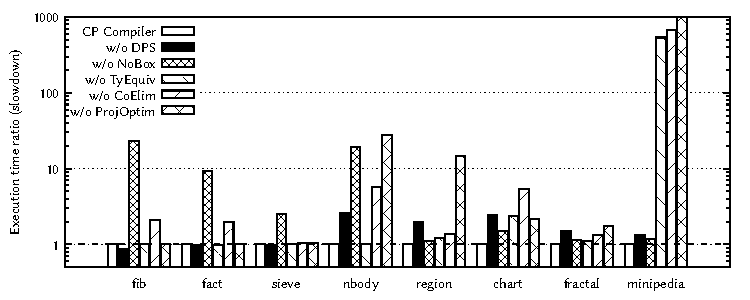
\includegraphics{benchmark1.pdf}
\caption{Execution time ratios (slowdowns) of different variants to the optimized JavaScript code.$^\ddagger$}
\footnotesize $^\ddagger$
The bar that exceeds the frame represents \emph{JavaScript heap out of memory} (OOM) for \textsf{minipedia w/o ProjOptim}.
\label{fig:benchmark1}
\end{subfigure}
\caption{Ablation study on optimizations for the CP compiler.}
\end{figure}

\noindent
We conduct an \emph{ablation study} on the four optimizations.
\autoref{fig:benchmark1} shows the execution time ratios (slowdowns) to the
optimized JavaScript code when removing each optimization.
\autoref{tab:benchmark1} lists the original data for \autoref{fig:benchmark1} in
milliseconds. \textsf{CP~Compiler} represents the most optimized version of the
CP compiler, including all the aforementioned optimizations. The remaining
variants are \textsf{CP~Compiler} minus one optimization, including all other
optimizations. To summarize the benchmark results, different optimizations show
different degrees of speedup for different benchmarks, but we believe that the
coercion-related ones are especially important when (dynamic) inheritance is
concerned.

The first optimization (\textsf{DPS}) speeds up the execution of the latter five
benchmarks by reducing the number of intermediate objects and object
concatenations. In contrast, the former three benchmarks do not benefit from the
optimization because they only perform arithmetic operations and no objects are
involved. The first benchmark (\textsf{fib}) even becomes a bit slower because
the optimization inserts extra checks into function bodies to test if
destination objects are present. Overall, the speedup ratios are 2.6$\times$ at
most. This optimization clearly helps for programs involving objects and
merging, although the benefits of this optimization are smaller than
optimizations on coercions. In essence, intermediate objects are not the main
bottleneck in the JavaScript code generated by the CP compiler, although they
still have a considerable cost for many programs.

The second optimization (\textsf{NoBox}) is important for primitive operations
such as arithmetic, which complements the first optimization. It speeds up all
benchmarks since primitive operations are inevitable in practical programs. It
brings around 23$\times$ speedup for \textsf{fib} and around 19$\times$ speedup
for \textsf{nbody} because they involve a lot of arithmetic operations. Numbers
do not need to be boxed/unboxed in the optimized JavaScript code, so the
performance is improved significantly.


The analysis for the third optimization is split into two parts for a
finer-grained analysis. We have a version of the CP compiler that only removes
coercions for \emph{syntactically equal} types but does not eliminate other
coercions for \emph{equivalent} types (\textsf{w/o TyEquiv}). The other version
does not eliminate redundant coercions at all (\textsf{w/o CoElim}). Some
benchmarks (such as \textsf{chart} and \textsf{minipedia}) make use of
equivalent types a lot, hence their performance is already affected by removing
\textsf{TyEquiv}. After further removing \textsf{CoElim}, most benchmarks
experience significant slowdowns (up to 671$\times$ slower in the worst case for
\textsf{minipedia}).

The last optimization (\textsf{ProjOptim}) targets coercions for record
projections, so the benchmarks that do not use records (such as \textsf{fib},
\textsf{fact}, and \textsf{sieve}) are not affected at all. Among the relevant
benchmarks, \textsf{nbody} becomes around 28$\times$ slower without this
optimization. This is because the masses, velocities, and coordinates of the
bodies are all stored in records. Note that the JavaScript code generated for
\textsf{minipedia} runs out of memory, so there is no data in
\autoref{tab:benchmark1}, and the exception is represented by a bar that exceeds
the frame in \autoref{fig:benchmark1}.

In conclusion, all optimizations work in practice. The elimination of redundant
coercions has a particularly significant impact on the performance. The
representation of JavaScript objects (or extensible records in general) brings
forth a class of equivalent types, whose terms share the same shape. We can then
avoid the coercions between these types but still obtain an equivalent object as
a result. This optimization has a significant impact but cannot be done in
previous work~\citep{dunfield2014elaborating,oliveira2016disjoint} because they
use nested pairs as the elaboration target of merges. Since pairs are
order-sensitive, they require coercions that can be avoided with
order-insensitive objects (see also the discussion in \autoref{sec:dunfield}).
Together with the faster lookup by type indices in objects, the JavaScript code
generated by the CP compiler achieves reasonable performance.

\section{Comparison with Handwritten JavaScript Code}

Our focus in this paper is on the type-safe compilation of dynamic inheritance
and the efficient compilation of languages with merges. A first natural question
to ask is how the new compilation scheme compares against existing compilation
schemes for merges. Unfortunately, such a direct comparison is not feasible for
a few different reasons. Firstly, the only other compiler for a language with
merges is Stardust by \citet{dunfield2014elaborating}. However, Stardust targets
ML, instead of JavaScript. Thus, a direct comparison of performance would not be
possible. Furthermore, Stardust does not support distributive subtyping and
nested composition. Thus, most of our examples and case studies cannot be
encoded in Stardust. Nevertheless, in \autoref{sec:dunfield}, we have
highlighted some advantages of using our record-based representation versus
using pairs (which Stardust employs) in the compilation of merges.  

In spite of the above-mentioned difficulties of a direct comparison, it is still
helpful to do an elementary quantitative analysis with handwritten JavaScript
code to assess the impact of the coercive semantics of CP. Although we have
worked hard to eliminate unnecessary coercions, the JavaScript code generated by
the CP compiler still includes plenty of coercions. In contrast, handwritten
JavaScript code is coercion-free, and subtyping in TypeScript has no cost. It
would be unrealistic to expect a stable performance that is competitive with
JavaScript, especially since our implementation is still a proof of concept for
our compilation scheme. However, ideally, the performance penalty imposed by
coercions should not be too high.

\begin{figure}
\begin{subfigure}{\textwidth}
\centering
\footnotesize
\begin{tabular}{r*{5}{c}}
& \sffamily fib & \sffamily fact & \sffamily sieve & \sffamily nbody & \sffamily region$^0$ \\
\toprule
\sffamily JavaScript & 2423 & 1427 & 1413 &  566 & 1513 \\
\sffamily CP         & 2837 & 1433 & 1736 & 1704 & 1137 \\
\bottomrule
\end{tabular}
\caption{Execution time (ms) for five benchmarks.} \label{tab:benchmark3}
\end{subfigure}
\begin{subfigure}{\textwidth}
\centering
\footnotesize
\bigskip
\begin{tabular}{r*{11}{c}}
Inheritance level & 0 & 1 & 2 & 3 & 4 & 5 & 6 & 7 & 8 & 9 & 10 \\
\toprule
\sffamily JavaScript & 1513 & 1896 & 2002 & 2328 & 2333 & 2515 & 2724 & 2928 & 3260 & 3507 & 3670 \\
\sffamily TypeScript & 1575 & 1944 & 2409 & 2755 & 3096 & 3614 & 4236 & 4606 & 4903 & 5186 & 5593 \\
\sffamily CP         & 1137 & 2184 & 2329 & 2465 & 2565 & 2708 & 2785 & 2873 & 2968 & 3069 & 3221 \\
\bottomrule
\end{tabular}
\caption{Execution time (ms) for \textsf{region}$^{0..10}$.} \label{tab:benchmark2}
\end{subfigure}
\begin{subfigure}{.5\textwidth}
\centering
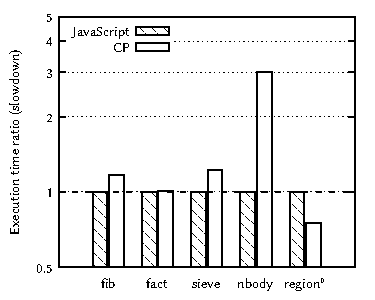
\includegraphics{benchmark3.pdf}
\caption{Bar chart for five benchmarks.}  \label{fig:benchmark3}
\end{subfigure}%
\begin{subfigure}{.5\textwidth}
\centering
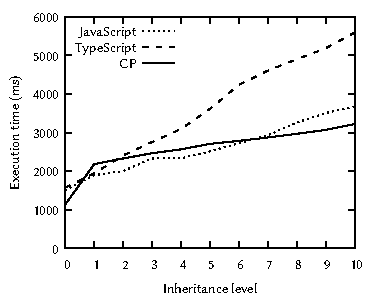
\includegraphics{benchmark2.pdf}
\caption{Line chart for \textsf{region}$^{0..10}$.}  \label{fig:benchmark2}
\end{subfigure}
\caption{Comparison between JavaScript code generated by the CP compiler and handwritten code.}
\end{figure}

A brief comparison is made based on the former four benchmarks, namely
\textsf{fib}, \textsf{fact}, \textsf{sieve}, and \textsf{nbody} (we will explain
\textsf{region}$^0$ later). \autoref{fig:benchmark3} shows the execution time
ratios (slowdowns) of the JavaScript code generated by the CP compiler compared
to the handwritten JavaScript code, and \autoref{tab:benchmark3} lists the
original data. They mainly demonstrate general-purpose computations. The
handwritten JavaScript code is transliterated from the corresponding CP code in
order to make an apples-to-apples comparison. It follows a functional
programming style similar to CP and may not be idiomatic in JavaScript. The
performance of the JavaScript code generated by the CP compiler is slightly
slower than that of the handwritten code for \textsf{fib}, \textsf{fact}, and
\textsf{sieve}. The biggest slowdown is around 3$\times$ for \textsf{nbody},
partly because the manipulations of records and arrays in CP are less efficient
than in native JavaScript. Moreover, our treatment of \lstinline{let}
expressions is oversimplified. In CP, \lstinline{let x = e1 in e2} is desugared
into \lstinline{(\x -> e2) e1}, which is much slower than
\lstinline[language=TypeScript]{const} statements in JavaScript. In
\textsf{nbody}, there are several nested \lstinline{let}s in recursive
functions, introducing significant overhead.

The latter four benchmark programs make use of CP's novel features, making
transliteration to JavaScript difficult. Nevertheless, we adapt the fifth
benchmark (\textsf{region}) to make a comparison between conceptually equivalent
programs. To recap, the benchmark program is mainly an embedded DSL for
geometric regions~\citep{hudak1998modular}. For modular extension, the DSL is
implemented with techniques of family polymorphism, which are described in
\autoref{sec:family} for JavaScript and in \autoref{sec:ep} for CP. Both
implementations heavily rely on class/trait inheritance, so the performance
penalty of inheritance is well demonstrated in this benchmark. Furthermore, we
change the number of inheritance levels from 0 to 10 (\textsf{region}$^n$
represents that the desired method is in the $n$-level super-trait/-class) to
see the trend of the performance penalty. In other words, \textsf{region}$^0$ is
\emph{monolithic} code with a single trait/class and no inheritance hierarchy.
At level one, we introduce a slightly more modular version of \textsf{region}
with one level of inheritance: there is a super-trait/-class and a
sub-trait/-class. Higher levels simply introduce more inheritance layers. The
results are shown in \autoref{tab:benchmark2} and \autoref{fig:benchmark2}.

Besides CP and JavaScript, a TypeScript version is also included for this
comparison. The source code is simply the JavaScript version plus type
annotations. We use the official TypeScript compiler to compile it to JavaScript
and then use Node.js to execute the JavaScript code. The TypeScript code has a
different performance profile from the JavaScript code because the TypeScript
compiler by default (as of the current version 5.4) desugars classes into
prototypes. This is due to the default compilation target being
ECMAScript~3~\citep{es3} for best compatibility, which does not support classes.
Newer versions of Node.js (based on ECMAScript~6~\citep{es6} or above) natively
support classes, so the handwritten JavaScript directly uses classes. To sum up,
the difference between JavaScript and TypeScript in the benchmark is mainly
classes versus prototypes. 

Without inheritance (\textsf{region}$^0$), the JavaScript code generated by the
CP compiler is \emph{faster} than the handwritten JavaScript and TypeScript
code. This is because the technique of nested anonymous classes is neither
idiomatic nor efficient in JavaScript. In contrast, nested traits themselves do
not introduce extra runtime overhead in CP. However, when the desired method is
one level up in the inheritance hierarchy, the CP compiler generates around
2$\times$ slower code, compared to the monolithic version, because coercions are
inserted for nested trait composition. For the monolithic version, there are
almost no coercions in the CP code. Then the performance penalty increases more
smoothly when the inheritance level is higher. The CP compiler regains its
leading position when the number of inheritance levels is higher than 6. In
contrast, TypeScript has the steepest curve. The desugared prototype-based code
generated by the TypeScript compiler is the least efficient among the three
implementations.

In conclusion, the performance penalty of coercions brought by trait inheritance
is not negligible but increases more smoothly with the number of inheritance
levels than in handwritten JavaScript. This is partly due to the efficient
lookup by type indices in extensible records (or, more specifically, JavaScript
objects). Looking up a deeply nested method in the inheritance hierarchy can be
slow in JavaScript, but this is not the case in CP.
